\documentclass[../ana1.tex]{subfiles}
\onlyinsubfile{\sectionNumbering} %Use numbering relative to sections and not subsection

\begin{document}
\setcounter{section}{18}
\section{Satz von Rolle, Mittelwertsatz, Extrema}
\begin{defi}[Lokale Extrema]
    Die Funktion \( f : [a,b] \rightarrow \R \) (oder \( (a,b) \))
    hat in \( x_0 \in [a,b] \) ein lokales Minimum (oder in 
    \( x_0 \in (a,b) \)), falls \( \exists \, \delta > 0 \), 
    sodass 
    \[ f(x_0) \leq f(x) \, \forall \, x \in U_\delta(x_0)
    \cap [a,b] = (x_0 - \delta, x_0 + \delta) \cap [a,b] \]
    Ist \( x_0 \in (a,b) \), so kann \( \delta > 0 \) so klein 
    gewählt werden, dass \( (x_0 - \delta, x_0 + \delta) 
    \cap [a,b] = (x_0 - \delta, x_0 + \delta) \).
    \begin{center}
    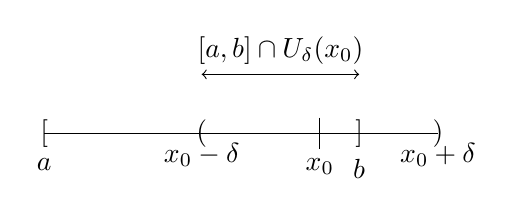
\begin{tikzpicture}
        \draw (0,0) -- (5,0);
        \draw (0,0) node {\([\)} node[below=2mm] {\(a\)};
        \draw (4,0) node {\(]\)} node[below=2mm] {\(b\)};
        \draw (3.5,0.2) -- (3.5,-0.2) node[below] {\(x_0\)};
        \draw (2,0) node {\((\)} node[below] {\( x_0 - \delta \)};
        \draw (5,0) node {\()\)} node[below] {\( x_0 + \delta \)};
        \draw[<->] (2,0.75) -- (4,0.75) node[midway,above] {\( [a,b] \cap U_\delta(x_0) \)};
    \end{tikzpicture}
    \end{center}
    Ist sogar \( f(x_0) < f(x) \,\forall \, x \in 
    (x_0 - \delta, x_0 + \delta) \cap [a,b] \), so heißt 
    das lokale Minimum isoliert (oder strikt).\\
    Analog: \( f \) hat in \( x_0 \) ein (indirektes) lokales 
    Maximum, falls \(-f\) in \(x_0\) ein (isoliertes) lokales 
    Minimum hat.\\
    Lokale Extrema \(=\) lokale Minima oder Maxima.
\end{defi}
\begin{satz}
    \( f: (a,b) \rightarrow \R \) habe in \(x_0 \in (a,b) \) 
    ein lokales Extremum. Ist \(f\) in \(x_0\) differenzierbar, 
    so gilt \( f'(x_0) = 0 \) (notwendige Bedingung für Extrema).
\end{satz}
\begin{bew}
    O.\ B.\ d.\ A.\ sei \(x_0\) ein lokales Minimum von \(f\) 
    (sonst betrachte \(-f\)).
    \[ \Rightarrow \exists \, \delta > 0 : f(x) \geq f(x_0) 
    \,\forall x \in (x_0 - \delta, x_0 + \delta) \]
    \[ \Rightarrow \frac{f(x) - f(x_0)}{x - x_0} = \begin{cases}
        \geq 0, &x \in (x_0, x_0 + \delta)\\
        \leq 0, &x \in (x_0 - \delta, x_0)
    \end{cases} \]
    \[ \Rightarrow f_+'(x_0) = \limesx{x}{x_0 +} 
    \frac{ f(x) - f(x_0) }{ x - x_0 } \geq 0 \]
    \[ = f_{\minus}'(x_0) = \limesx{x}{x_0 \minus} 
    \frac{ f(x) - f(x_0) }{ x - x_0 } \leq 0 \]
    \[ \Rightarrow f'(x_0) = f_{\pm}'(x_0) = 0. \]
    Rand: \(f: [a,b] \rightarrow \R \) \\
    hat lokales Minimum bei \( x_0 = b \).
    \[ \Rightarrow \frac{ f(x) - f(b) }{ x - b } \leq 0 \]
    \[ \Rightarrow f_{\minus}'(b) \leq 0. \]
\end{bew}
\begin{satz}[Rolle]
    Sei \( f: [a,b] \rightarrow \R \) stetig und differenzierbar 
    in \( (a,b) \) mit \( f(a) = f(b) = 0 \).
    \[ \Rightarrow \exists \, \xi \in (a,b) : f'(\xi) = 0. \]
\end{satz}
\begin{bew}
    \( [a,b]\) ist kompakt und \(f\) ist stetig.
    \[ \Rightarrow \exists \, \xi_1 \in [a,b], \xi_2 \in [a,b]: \]
    \[ f(\xi_1) = \sup( f(x), x \in [a,b] ), f(\xi_2) 
    = \inf (f(x) : x \in [a,b]). \]
    \( \Rightarrow \) Ist \( \xi_1 \in (a,b) \), nehme 
    \( \xi := \xi_1 \overset{\text{Satz 2}}{\Rightarrow}
     f'(\xi) = 0 \).\\
    Ist \( \xi_2 \in (a,b) \), nehme \( \xi := \xi_2 \)
    \( \oversett{Satz 2}{\Rightarrow} f'(\xi) = 0 \).\\
    Sind \( \xi_1, \xi_2 \in [a,b] \)
    \[ \sup(f(x) : x\in [a,b]) = \inf(\ldots) = 0. \]
    Also ist \( f(x) = 0 \,\forall \, x\in [a,b] \)
    \[ \Rightarrow f'(x) = 0 \, \forall \, x\in (a,b). \]
\end{bew}
\begin{satz}[Mittelwertsatz]\label{satz:mittelwert}
    \( f: [a, b] \rightarrow \R \) stetig und differenzierbar 
    auf \((a,b)\).
    \[ \Rightarrow \exists \, \xi \in (a,b): f'(\xi) = \frac{f(b)-f(a)}{b-a} \]
\end{satz}
\begin{bew}
    \( h(x) :=  f(x) - \left[f(a) + \frac{f(b)-f(a)}{b-a} 
    \cdot (x-a) \right] \) \\
    \( \Rightarrow h: [a,b] \rightarrow \R \) stetig und 
    differenzierbar auf \( (a,b) \) und 
    \[ h(a) = 0 = h(b) \oversett{Rolle}{\Rightarrow} 
    \exists \, \xi \in (a,b): 0 = h'(\xi) = f'(\xi) 
    - \frac{f(b)-f(a)}{b-a} \]
    \[ \Rightarrow f'(\xi) = \frac{f(b)-f(a)}{b-a}. \]
\end{bew}
\begin{kor}[Monotoniekriterium]\label{satz:monotoniekrit}
    Sei \( f : [a,b] \rightarrow \R \) stetig und differenzierbar 
    auf \( (a,b) \).\\
    Dann gilt:
    \begin{align*}
        f'(x) = 0 \,\forall \, x \in (a,b) \Leftrightarrow 
        f \text{ ist konstant auf } [a,b].\\
        f'(x) \geq 0 \,\forall \, x \in (a,b) \Leftrightarrow 
        f \text{ ist wachsend auf } [a,b].\\ 
        f'(x) \leq 0 \,\forall \, x \in (a,b) \Leftrightarrow 
        f \text{ ist fallend auf } [a,b].\\
    \end{align*}
    Strikte Ungleichungen implizieren strenge Monotonie auf 
    \( [a,b] \).
\end{kor}
\begin{bew}
    \[ \overref{satz:mittelwert}{MWS}{\Rightarrow} \exists \, 
    \xi \in (x_1, x_2) \text{ mit } \]
    \[ f(x_2) - f(x_1) = f'(\xi) \underbrace{(x_2 - x_1)}_{>0}
    = \begin{cases}
        =0, & \text{falls } f'(\xi) = 0\\
        \geq 0 &\text{falls } f'(\xi) \geq 0\\
        > 0 &\text{falls } f'(\xi) > 0\\
        \leq 0 &\text{falls } f'(\xi) \leq 0\\
        < 0 &\text{falls } f'(\xi) < 0
    \end{cases}. \]
\end{bew}
\begin{kor}[Schrankensatz]\label{satz:schranken}
    Sei \( f: [a,b] \rightarrow \R \) stetig und differenzierbar 
    auf \( (a,b) \).\\
    Dann gilt für \( a \leq x_1 < x_2 \leq b \): 
    \begin{enumerate}
        \item \( f'(x) \geq m \,\forall \, x \in (a,b) 
        \Rightarrow f(x_2) - f(x_1) \geq m(x_2 - x_1) \).
        \item \( f'(x) \leq M \, \forall \, x\in (a,b) 
        \Rightarrow f(x_2) - f(x_1) \leq M(x_2 - x_1) \).
    \end{enumerate}
\end{kor}
\begin{bew}
    Sei \( g(x) = m(x) \).
    \[ \Rightarrow (f - g)' = f' - g' \geq m - m = 0. \]
    \( \oversett{\autoref{satz:monotoniekrit}}{\Rightarrow} 
    f - g \) ist wachsend \dphp{} \( f(x_2) - m x_2 \geq 
    f(x_1) - m x_1 \) 
    \[ \Rightarrow f(x_2) - f(x_2) \geq m x_2 - m x_1 
    = (x_2 - x_1)m. \]
    Andere analog.
\end{bew}
\begin{bsp}%BSP 3???
    Achtung. Mittelwertsatz gilt nicht für 
    vektorwertige Funktionen
    \[ f: [a,b] \rightarrow \R^d, d \geq 2. \]
    z.B. \( f(x) = (x^2,x^3) \) auf \( [0,1] \). \\
    Angenommen, \( \exists \, \xi \in (0,1) \) mit 
    \[ (2\xi, 3\xi^2) = f'(\xi) = \frac{f(1) - f(0)}{1-0} 
    = f(1) = (1,1) \]
    \[ \Rightarrow 2\xi = 1 \text{ und } 3\xi^2 = 1 \text{ \Lightning{}} \]
    Problem: Für die einzelnen Komponenten kann nicht die selbe Stelle 
    \( \xi \) gewählt weden!\\
    Trotzdem gilt eine vektorwertige Version des Schrankensatzes.    
\end{bsp}
\begin{kor}[\( f' \) beschränkt \( \Rightarrow f \) Lipschitzstetig]
    Sei \( f: [a,b] \rightarrow \R^d \) stetig und 
    differenzierbar auf \( (a,b) \). \\
    Gilt \( ||f'(x)|| \leq L \, \forall \, x \in (a,b) \), 
    so folgt 
    \[ ||f(x) - f(y)|| \leq L ||x-y|| 
    \; \forall \, x,y \in [a,b] \]
\end{kor}
\begin{bew}
    Übung.
\end{bew}
\begin{prosa}
    Achtung: All das geht schief, wenn man nicht auf 
    \( \R \) arbeitet.
    \[ \text{z. B. } f: \Q \rightarrow \Q, x \mapsto 
    \begin{cases}
        1, x^2 > 2\\
        -1, x^2 < 2
    \end{cases} \]
    ist stetig und differenzierbar mit 
    \( f'(x) = 0 \; \forall \, x \in \Q \), aber 
    \( f \) ist nicht konstant (Monotoniesatz) \Lightning{}.
    \( g: \Q \rightarrow \Q, x \mapsto g(x) = x + f(x) \) 
    ist differenzierbar mit \( g'(x) = 1 > 0 \), aber 
    \( g \) ist nicht monoton wachsend.
\end{prosa}
\begin{defi}
    Die \( k \)-te Ableitung von 
    \( f: (a,b) \rightarrow \R \) in \( x_0 \) ist 
    induktiv definiert durch 
    \[ f^{(k)}(x_0) = (f^{(k-1)})'(x_0). \]
    Damit \( f^{(k)}(x_0) \) definiert ist, müssen 
    also die Ableitungen bis \( (k-1) \)-ter Ordnung 
    in einer Umgebung von \( x_0 \) definiert sein und 
    \( f^{(k-1)} \) muss in \( x_0 \) differenzierbar sein.
\end{defi}
\begin{notation}
    Schreiben \( f' \) für \( f^{(1)} \) und \( f'' \) 
    für \( f^{(2)} \).
\end{notation}
\begin{satz}
    Sei \( f: (a,b) \rightarrow \R \) differenzierbar. \\
    Ist \( x_0 \in (a,b) \) und gelte 
    \[ f'(x_0) = 0 \text{ und } f''(x_0) \text{ existiert.} \]
    Dann gilt:
    \begin{enumerate}
        \item Ist \( f''(x_0) > 0 \), so hat \( f \) in 
        \( x_0 \) ein isoliertes lokales Minimum.
        \item Hat \( f \) in \( x_0 \) ein lokales 
        Minimum, so folgt \( f''(x_0) \geq 0 \).
    \end{enumerate}
    Analoge Aussagen mit umgekehrten Ungleichungen gelten 
    für Maxima.
\end{satz}
\begin{bew}
    Da \( f'(x_0) = 0 \) gilt 
    \[ f''(x_0) = \limesx{x}{x_0} 
    \frac{f'(x) - f'(x_0)}{x - x_0} 
    = \limesx{x}{x_0} \frac{f'(x)}{x - x_0}. \]
    Unter der Voraussetzung 1. gibt es also ein 
    \( \delta > 0 \) mit 
    \begin{align*}
        &f'(x) < 0 \text{ auf } (x_0 - \delta, x_0) \\
        &f'(x) > 0 \text{ auf } (x_0, x_0 + \delta)        
    \end{align*}
    \begin{align*}
        \overref{satz:monotoniekrit}{Kor.\ 5}{\Rightarrow} 
        &f \text{ ist streng}
        \text{monoton fallend auf } (x_0 - \delta, x_0) \\
        &f \text{ ist streng monoton wachsend auf }
        (x_0, x_0 + \delta) \\
        \Rightarrow \, &f \text{ hat in } x_0
        \text{ ein isoliertes lokales Minimum.}                                        
    \end{align*}
    Wäre in 2. \( f'(x_0) < 0 \), so hätte \( f \) nach 1. 
    ein isoliertes lokales Maximum \Lightning{} \( f \) hat 
    in \(x_0\) ein lokales Minimum.
\end{bew}
\begin{bsp}[Young'sche Ungleichung]
    Für alle \( x,y \geq 0 \) und \( p,q \in (1,\infty) \) 
    mit 
    \[ \frac{1}{p} + \frac{1}{q} = 1 \]
    gilt
    \[ xy \leq \frac{x^p}{p} + \frac{y^q}{q}. \]
\end{bsp}
\begin{bew}
    Die Ungleichung gilt sicherlich falls \( x=0 \) oder 
    \( y = 0 \). \\
    Sei \( y > 0 \) und \( f_y(x) := xy - \frac{x^p}{p} \). \\
    Da \( x^p = \exp(p \cdot \ln x) \)
    \begin{align*}
        \Rightarrow (x^p)' &= \exp'(p \cdot \ln x)
        \cdot \frac{p}{x} = \exp(p \cdot \ln x) 
        \cdot \frac{p}{x} \\
        &= x^p \frac{p}{x} \\
        &= p \cdot x^{p-1} \; (x>0)        
    \end{align*}
    \[ \text{und } (x^p)'' = p (p-1) x^{p-2} > 0 
    \text{ für } x > 0, p > 1. \]
    \[ \limesx{x}{0} f_y(x) = 0, \qquad 
    \limes{x} f_y(x) = -\infty \]
    \[ \text{und } f_y(x) = x\left( y 
    - \frac{x^{p-1}}{p} \right) >0 
    \text{ falls } x>0 \text{ klein genug ist.} \]
    Somit gilt, da \( [0,\infty) \ni x \mapsto f_y(x) \) 
    stetig ist, hat es mindestens ein positives Maximum für 
    \( x > 0 \).
    \begin{align*}
        f_y'(x) = 0 &\Leftrightarrow y - x^{p-1} = 0 \\
        &\Leftrightarrow x = y^{\frac{1}{p-1}} \\
        M_y = f_y(f^{\frac{1}{p-1}}) 
        &= y \cdot y^{\frac{1}{p-1}} 
        - \frac{ (y^{\frac{1}{p-1}})^p }{ p } \\
        &= (1- \frac{1}{p}) y^{\frac{p}{p-1}} 
        = \frac{1}{q} y^q \\
        \left( \text{Bemerkung: da } \frac{1}{q} = 1 - \frac{1}{p} \right) \\ 
        &= \frac{p}{p-1}
    \end{align*} 
    Außerdem ist 
    \[ f_y''(x) = -p(p-1)x^{p-2} < 0 \]
    für alle \( x > 0 \).\\
    \( \Rightarrow \) Bei \( x = y^{\frac{1}{p-1}} \), hat 
    \( f_y \) das einzige Maximum und da 
    \( 0 = \limesx{x}{0} f_y(x) \) und 
    \( -\infty = \limesx{x}{\infty} f_y(x) \), ist 
    \[ M_y = f_y \left( y^{\frac{1}{p-1}} \right) 
    = \frac{y^q}{q} \] 
    das globale Maximum für \( f_y \) auf \( (0,\infty) \).

    \begin{align*}
        xy &= \frac{x^p}{p} + \underbrace{xy - \frac{x^p}{p}}_{
            = f_y(x)
        } \\
        &\leq \frac{x^p}{p} + \underset{x>0}{\sup} f_y(x) 
        = \frac{x^p}{p} + M_y \\
        &= \frac{x^p}{p} + \frac{y^q}{q}.
    \end{align*}
\end{bew}
\begin{bem}
    Ist \( F: [0,\infty) \rightarrow \R \) mit 
    \[ F(0) = \limesx{x}{0} F(x), 
    \limes{x} \frac{F(x)}{x} = \infty. \]
    Setze \( G(y) := \underset{x>0}{\sup} (xy - F(x)) \)
    \[ \Rightarrow xy \leq F(x) + G(y) 
    \; (\text{z. B. } F(x) = e^x - 1) \]
    \[ (xy - (e^x - 1))' = y - e^x \overset{!}{=} 0 
    \Leftrightarrow x = \ln y \]
    falls \( y \geq 1 \) \\
    Ist \( 0 \leq y < 1 \Rightarrow y - e^x < 1 
    \, \forall x \geq 0 \) \\
    \( \Rightarrow \) globales Maximum bei \( x=0 \). \\
    \begin{align*}
        \text{Insgesamt } x &= (\ln y)_+ = \begin{cases}
            \ln y, y \geq 1 \\
            0, 0 \leq y < 1
        \end{cases} \\
        &\Rightarrow G(y) = ( \ln y )_+ - (e^{(\ln y)_+} - 1) \\
        &= \begin{cases}
            y \ln y - y + 1, &1 \leq y \\
            y \cdot 0 - e^0 + 1, &0 \leq y < 1
        \end{cases} \\
        &= \begin{cases}
            y (\ln y - 1) + 1, &1 \leq y \\
            0, &0 \leq y < 1
        \end{cases} \\
        &= y (\ln y - 1) + 1 \; \forall \, x,y \geq 0        
    \end{align*}
    \[ \Rightarrow xy \leq e^x - 1 + y^{(\ln y + 1)_+} + 1
    = e^x + y^{(\ln y - 1)_+} \]
\end{bem}
\end{document}